\documentclass{article}
\usepackage{graphicx}
\graphicspath{ {./grafiki/} }
\usepackage{transparent}
\usepackage[T1]{fontenc}
\usepackage[a4paper, total={15cm, 24cm}]{geometry}
\usepackage[polish]{babel}
\usepackage{amssymb}
\usepackage{amsmath}
\usepackage[
  pdfpagelabels=true,
  pdftitle={Notatki z OWI},
  pdfauthor={Jan Pulkowski},
  colorlinks=true,
  linkcolor=blue,
  ]{hyperref}
\usepackage[]{titlesec}
\usepackage[p]{scholax}

\setcounter{secnumdepth}{2}

\renewcommand{\thesection}{\arabic{section}}

\titleformat{\section}{\normalfont\Large\bfseries\scshape}{Wykład \thesection:}{1em}{}

\title{Notatki z Ochrony Własności Intelektualnej}
\author{mlecz}
\date{Semestr Letni 2024}

\begin{document}

\maketitle
\tableofcontents

\section{Prawo i jego źródła}

\subsection{Prawo}

\paragraph{Prawo w ujęciu normatywnym}

to zespół norm i reguł określających postępowanie ludzi, ustanowionych, usankcjonowanych i zabezpieczanych przez aparat przymusu państwowego.

\paragraph{Prawo wg Kanta}

to reguły pozwalające na pogodzenie samowoli dwóch niezależnych jednostek.

\subsubsection{Zasady Prawa}

\begin{itemize}
  \item Lex posterior derogat legi priori -- prawo późniejsze uchyla prawo wcześniejsze
  \item Lex superiori derogat legi inferiori -- prawo o wyższej mocy uchyla prawo o niższej mocy
  \item Lex specialis derogat legi generali -- prawo szczegółowe uchyla prawo ogólne
  \item Ne bis in idem -- Nie można orzekać dwa razy w tej samej sprawie
  \item Lex retro non agit -- Prawo nie działa wstecz (o ile ustawa późniejsza nie jest
        korzystniejsza dla oskarżonego)
\end{itemize}

\subsubsection{Miejsca zapisu prawa}

\begin{itemize}
  \item \textbf{Dziennik ustaw -- jedyne oficjalne miejsce zapisu prawa}
  \item Monitor Polski -- służy do ogłaszania wewnętrznych aktów prawnych wydawanych
        przez~organy państwowe
  \item ISAP -- Internetowy System Aktów Prawnych
  \item Systemy Prawne (LEX, Legalis) -- ujednolicony i czytelny zapis informacji
        z dziennika ustaw z odnośnikami do innych powiązanych informacji prawnych
\end{itemize}

\subsection{Język prawny a prawniczy}

\paragraph{Język prawny}

to język tworzenia prawa, w którym tworzone są akty prawne.
Nie musi być~poprawny w sensie składni j. pol. ale jest mniej wieloznaczny i ściślejszy
od języka naturalnego.

\paragraph{Język prawniczy}

to język stosowania i doktryny prawa, omawiający treść
i interpretację ustawy.

\paragraph{Język prawny a matematyczny}

Język prawny często celowo zostawia pewne pojęcia niedookreślone,aby pozostawić
sądom pole do odmiennej wykładni prawa w różnych przypadkach.

\subsection{Obowiązywanie Prawa}

\paragraph{Prawo powszechnie obowiązujące}

to przepisy adresowane do wszystkich podmiotów.
Wyznacza ich sytuację prawną, tzn. prawa i obowiązki.
Stanowi fundament działania państwa,
jest umową społeczną między jego państwa i obywatelami.

Państwo może wykonywać jedynie czynności \textit{explicite} dozwolone przez prawo,
a obywatele wszystkie czynności niezakazane.

\subsection{Źródła prawa}

Uszeregowane według malejącej mocy:
\begin{enumerate}
  \item Konstytucja
  \item Ratyfikowane umowy międzynarodowe
  \item Ustawy
  \item Rozporządzenia
  \item Akty prawa miejscowego (tylko na obszarze obowiązywania)
\end{enumerate}

\paragraph{Konstytucja}

akt prawny nadrzędny wobec wszystkich pozostałych.
Jej przepisy stosuje się bezpośrednio, o ile sama nie stanowi inaczej.
Jest jednym, spójnym aktem prawnym. Konstytucja jest celowo napisana w sposób ogólny, aby mogły
uszczegółowić ją ustawy.
Określa bazowe ramy prawne, sposób stanowienia prawa i zasady jakie można z niej wyprowadzać.

\paragraph{Ustawa, a rozporządzenie}

Ustawa to prawo stanowione przez władzę ustawodawczą,
rozporządzenie jest aktem wykonawczym, doprecyzowuje działanie i stosowanie ustawy oraz określa
szczegółowe procedury jej realizacji. Rozporządzenia są tworzone na podstawie ustaw.

\subsection{Prawo unijne}

\paragraph{Prawo pierwotne}
to umowy międzynarodowe tworzące i kształtujące Unię Europejską. Stanowią jej swoistą konstytucję.
Na przykład Traktat z Lizbony powołujący Unię.

\paragraph{Prawo wtórne}
to rozporządzenia, dyrektywy, decyzje, opinie i zalecenia wydawane przez~organy Unii.

\paragraph{Rozporządzenia unijne} to akty prawne
bezpośrednio i jednolicie działające we wszystkich krajach członkowskich.

\paragraph{Dyrektywy unijne} to akty prawne,
wskazujące cele i wytyczne, które ustawodawstwo poszczególnych krajów członkowskich powinno zrealizować.
Muszą zostać wydane krajowe akty prawne, które implementują dyrektywę.

\subsubsection{Prawo polskie a prawo unijne}
Konstytucja dopuszcza przekazanie części uprawnień organów państwowych organom prawa międzynarodowego.
Proeuropejska wykładnia prawa jest ponad krajową --
ratyfikowana umowa międzynarodowa ma pierwszeństwo wobec sprzecznej z nią ustawy.
Nad umowami międzynarodowymi stoi jedynie konstytucja.

\newpage

\section{Własność Intelektualna}

\subsection{Dobra Niematerialne}

\paragraph{Dobro niematerialne (intelektualne)}

to wytwór myśli, cechujący się twórczym charakterem, istniejący w świadomości człowieka
i mogący podlegać ochronie prawnej niezależnie od~swojego ewentualnego nośnika \textit{(Corpus Mechanicum)}.

\subsubsection{Rodzaje dóbr niematerialnych}

\begin{itemize}
  \item Utwory (w rozumieniu prawa autorskiego)
  \item Rozwiązania -- zaplanowane koncepty, prowadzące do realizacji danego celu (wynalazki, projekty, wzory)
  \item Oznaczenia, symbole (znaki towarowe, oznaczenia geograficzne)
\end{itemize}

Dobra niematerialne mogą obejmować więcej niż jeden z powyższych aspektów.

\subsection{Prawo własności intelektualnej}

\paragraph{Prawo autorskie i pokrewne}

zajmuje się utworami. Godzi prawa twórców z możliwością rozwoju społeczeństwa. Chroni prawa twórców jak i wykonawców. Regulowane międzynarodowo.

\subsection{Konwencje o ochronie prawa autorskiego}

\subsubsection{Konwencja Berneńska}

\paragraph{Konwencja Berneńska}

o ochronie dzieł literackich i artystycznych z 1886 roku. Powstała z~inicjatywy m. in. Wiktora Hugo.
Wprowadziła koncept międzynarodowej ochrony praw autora.
Ratyfikowana przez większość państw świata, wielokrotnie nowelizowana. Nadal obowiązuje.

\paragraph{Zasada wzajemnego respektowania praw}

Utworom zagranicznym zapewnia się taką samą ochronę jak utworom krajowym.

\paragraph{Zasada automatyzmu}

Ochrona praw autorskich przysługuje każdemu utworowi od momentu jego powstania.

\subsubsection{Inne Konwencje}

\paragraph{Konwencja genewska}

o prawach autorskich.
Zapewnia alternatywę wobec Konwencji Berneńskiej.
Reprezentuje bardzie liberalne podejście do sprawy.

\paragraph{Konwencja Rzymska}

o ochronie wykonawców, producentów fonogramów oraz organizacji nadawczych.
Zapewnia ochronę twórcom utworów dźwiękowych.

\paragraph{Porozumienie w sprawie Handlowych Aspektów Praw Własności Intelektualnej (TRIPS)}

poza zakresem Konwencji Berneńskiej zapewniło ochronę programów komputerowych i~baz~danych.
Chroni programy w postaci kodu źródłowego i przedmiotowego (postać binarna, wynikowa, ang. \textit{object files}). Polska przystąpiła do niego w 1995 roku.

\paragraph{Traktaty Światowej Organizacji Własności Intelektualnej (WIPO)}

o prawie autorskim, o artystycznych wykonaniach i fonogramach.
Pierwszy traktat międzynarodowy nakładający obowiązek chronienia programów komputerowych i baz danych.
Wymusza wprowadzenie sankcji za łamanie i obchodzenie zabezpieczeń programów.

\subsection{Ustawa o prawach autorskich i pokrewnych}

\subsubsection{Utwory}

\paragraph{Utwór}

to każdy przejaw działalności twórczej o indywidualnym charakterze, ustalony w~jakiejkolwiek postaci,
niezależnie od wartości, przeznaczenia i sposobu wyrażenia.
Definicja celowo jest szeroka aby móc pozostawić kwestię, czy dana rzecz jest utworem do interpretacji sądowej.

\paragraph{Konkretne przypadki wykładni definicji utworu}

\begin{itemize}
  \item Smak i zapach nie może podlegać ochronie prawnoautorskiej. Subiektywne doznania odgrywają tu zbyt dużą rolę.
  \item By mówić o utworze konieczna jest cecha nowości, twórca musiał wprowadzić uchwytne elementy, nieobecne w dotychczasowym stanie rzeczy.
  \item Jeżeli wysoce prawdopodobne jest, że ktoś w przyszłości wytworzy \textbf{identyczny} przedmiot, to nie mówi się o utworze.
\end{itemize}

\paragraph{Zasada Ustalenia}

Utwór musi zostać przedstawiony, w postaci która pozwala na jego percepcję komuś innemu niż twórcy, nawet ulotnej, nietrwałej.
Utwór może istnieć bez nośnika, a posiadanie nośnika nie jest związane z prawem do utworu.

\newpage

\section{Twórcy i ochrona utworów}

\subsection{Osoba twórcy}

\paragraph{Twórcą}

utworu może być dowolna osoba, niezależnie od stanu świadomości.
W porządku prawnym amerykańskim i polskim przesądzono, że zwierzęta ani natura nie mogą być twórcą utworu.
Ogólnie, twórcą może być wyłącznie człowiek.
Często uważa się, że wytwory systemu niedeterministycznych (np. AI) należą do ich operatorów,
natomiast nie jest to uniwersalna wykładnia i silnie zależy od konkretnego przypadku.
Obecny porządek prawny niedostatecznie określa interpretacje praw do wytworów sztucznej inteligencji,
która nie może być uznana za~twórcę utworu.

\subsection{Ochrona utworów}

Utwór jest chroniony od momentu powstania, nawet w postaci nieukończonej.
Ochrona przysługuje mu niezależnie od spełnienia jakichkolwiek formalności.
Ochronie nie może podlegać procedura, koncepcja matematyczna ani odkrycia,
a jedynie sposób wyrażenia (nie temat a jego indywidualizacja).
Dyrektywy unijne i inne przepisy doprecyzowują kryteria uznania tworu konkretnego typu za utwór.

\subsubsection{Czy każde dzieło jest chronione jako utwór?}

tldr.: Nie.

\begin{figure}[h]
  \begin{minipage}{0.31\textwidth}
    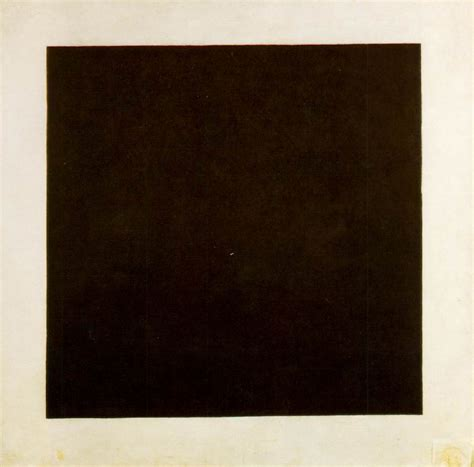
\includegraphics[width=0.95\textwidth]{malewiczkwadrat}
    \caption{K. Malewicz -- Czarny kwadrat na białym tle}\label{fig:malewiczkwadrat}
  \end{minipage}
  \hfill
  \begin{minipage}{0.31\textwidth}
    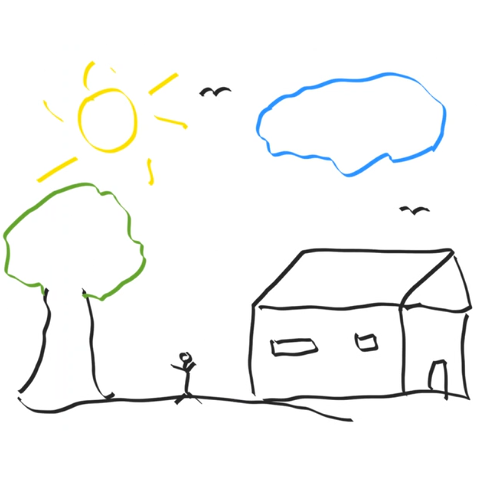
\includegraphics[width=0.95\textwidth]{behandomek}
    \vspace{-\baselineskip}
    \caption{A. Behan -- 2023}\label{fig:behandomek}
  \end{minipage}
  \hfill
  \begin{minipage}{0.31\textwidth}
    
\includegraphics[width=0.95\textwidth]{iosononiewidzialne}
    \vspace{-\baselineskip}
     \caption{S. Garau -- Io Sono}\label{fig:iosononiewidzialne}
  \end{minipage}
\end{figure}

Z powyższych utworem jest tylko Rysunek 2.
Niewidzialna rzeźba (3) istnieje jedynie jako~koncepcja, nie ma żadnej ustalonej formy -- nie jest utworem.
Natomiast czarny kwadrat (1) pomimo oryginalnej koncepcji, nie spełnia kryterium oryginalności.
Prawdopodobieństwo wytworzenia identycznego dzieła jest zbyt duże by mówić o utworze.

\subsection{Ochrona programów komputerowych}

\paragraph{Programy Komputerowe}

podlegają ochronie w każdej postaci (kod, kod skompilowany, zapis na nośniku).
Program chronią też wystarczająco szczegółowe prace przygotowawcze i projektowe.
Ochrona to nie zależy od testów jakościowych ani estetycznych programu, ani~od~jego~oryginalności.

Programy komputerowe są chronione w taki sam sposób co dzieła literackie.
Natomiast, nie~są~chronione ich koncepcje i interfejsy (graficzne/tekstowe), ale pojedyncze elementy programów mogą być chronione z osobna.
Np. interfejs graficzny może być objęty ochroną utworu, ale osobno od ochrony samego programu komputerowego.

\subsubsection{Dekompilacja Programów Komputerowych}

\paragraph{Interfejs}

logiczna lub fizyczna część systemu informatycznego, służąca komunikacji z~jego~innymi częściami i użytkownikami.

\paragraph{Interoperacyjność}

umożliwienie połączenia, współpracy i oddziaływania pomiędzy interfejsami.
Zdolność do wymiany informacji i wykorzystania informacji już wymienionych.

\paragraph{Dekompilacja}

tłumaczenie formy programu komputerowego do wersji wyższego poziomu, termin nie jest jednoznaczny z informatycznym. Jest dozwolona jeżeli służy osiągnięciu interoperacyjności danego programu z innymi.

\paragraph{Kto może dekompilować?}

Osoba będące licencjobiorcą, posiadające prawo do używania kopii programu, lub działająca w imieniu takich osób.

\paragraph{Kiedy można dekompilować?}

Gdy informacje konieczne do osiągnięcia interoperacyjności nie są łatwo dostępne i nie jest na celu naruszenie uzasadnionych interesów twórców programu ani wykorzystanie programu w celach innych niż standardowe.

Poprawienie błędu i naprawy są uzasadnionym powodem.
Nie jest wymagane zezwolenie autora i nie wolno zabraniać napraw.


\section{Autorskie prawa zależne}

\subsection{Utwory zależne}

\paragraph{Utwór zależny}

opracowanie utworu pierwotnego takie jak tłumaczenie, przeróbka, adaptacja.

Utwory zależne można tworzyć i rozpowszechniać jedynie za zgodą pierwotnego twórcy, ale~jeśli jego prawa wygasły to zgoda nie jest wymagana.
Wytworzenie ich jest bez uszczerbku dla praw pierwotnych i pociąga za sobą prawa autora utworu zależnego.
Należy zaznaczyć, że~jest to utwór zależny oraz wymienić twórcę i tytuł utworu pierwotnego.


\paragraph{Tłumaczenia}

nie zawsze noszą cechy utworów -- tłumaczenia które mają w sobie mało inwencji,
jak np. tłumaczenia dokumentacji technicznej nie są utworami, w przeciwieństwie do~np.~tłumaczeń dzieł literackich.

\paragraph{Utwory zależne a inspirowane}

Utwór inspirowany to taki, który zawiera pewne motywy zawarte w innym utworze.
Jeżeli motywy są zindywidualizowane do postaci zawartej w utworze pierwotnym, to nie jest to już utwór inspirowany.
Utwory inspirowane nie są utworami zależnymi

\section{Utwory niechronione prawem autorskim}

Poniższe kategorie utworów są niechronione prawem autorskim,
mogą natomiast być chronione jako symbole narodowe, znaki towarowe bądź przez inne akty prawne.

\begin{itemize}
  \item akty normatywne i ich projekty
  \item urzędowe dokumenty, materiały, znaki i symbole
  \item opublikowane opisy patentowe, lub ochronne
  \item proste informacje prasowe (informacje zawierające same fakty, bez elementu twórczego)
\end{itemize}

Nie wszystkie materiały tworzone przez urzędy to materiały urzędowe.
Na przykład dokumenty wytworzone na potrzeby przetargów, jak najbardziej są chronione prawem autorskim.

\section{Podmiot prawa autorskiego}

\subsection{Komu przysługują prawa autorskie?}

Prawa autorskie przysługują twórcy, o ile ustawa nie stanowi inaczej (utwory zbiorowe, lub~pracownicze).
Domniemywa się, że twórcą jest osoba, której autorstwo podano do publicznej wiadomości wraz z rozpowszechnianiem utworu.
Twórca nie musi ujawniać swojego autorstwa, wówczas w wykonywaniu prawa autorskiego zastępuje go wydawca, lub odpowiednia organizacja zbiorowo zarządzająca prawami autorskimi.

\subsection{Czy można odstąpić od praw autorskich?}

Ogólnie, nie można odstąpić praw innej osobie, jednak istnieją szczególne przypadki, na~które~pozwala ustawa.

\subsection{Utwory zbiorowe}

W przypadku utworu zbiorowego prawa autorskie do całości i tytułu przysługują wydawcy, natomiast do jego poszczególnych elementów, ich twórcom.

\subsubsection{Programy komputerowe}

Ogólnie są rozpatrywane jak utwory zbiorowe, jednak, jeśli powstają w wyniku wykonywania obowiązków wynikających ze stosunku pracy, prawa do nich przysługują pracodawcy, o~ile~umowa nie stanowi inaczej.

\subsubsection{Współtwórczość}

Współtwórcom przysługują wspólne prawa autorskie, wielkości udziałów są równe, o ile sąd, na wniosek współtwórcy, nie orzecze inaczej.
Każdy współtwórca może bez uszczerbku dla~innych wykonywać prawa autorskie do swojej części utworu,
ale do wykonania prawa autorskiego do całości utworu konieczna jest zgoda wszystkich współtwórców, w przypadku braku zgody rozstrzyga sąd.
Każdy ze współtwórców może dochodzić roszczeń w sprawie naruszenia praw do całości utworu.

Za współtwórcę uznaje się osobę, która włożyła w utwór działanie intelektualnej o twórczym charakterze, współtwórcy muszą działać w porozumieniu.
Pomysłodawca nie jest współtwórcą i nie można zostać współtwórcą wyłącznie na podstawie umowy.

\subsection{Utwory pracownicze}

Prawa majątkowe i zależne do utworów tworzonych na podstawie obowiązków wynikających ze stosunku pracy przechodzą na pracodawcę w chwili przyjęcia utworu (rozpoczęcia jego wykorzystywania), o ile UoP nie stanowi inaczej.
Nie można zawrzeć takiej umowy co do wszystkich utworów tworzonych w przyszłości przez twórcę.

Utwory tworzone podczas konkursów, o ile ich regulamin nie stanowi inaczej, nie mają charakteru pracowniczego.

\newpage

\subsubsection{Umowy o pracę, a cywilnoprawne}

Rozróżniają stosunek pracy od stosunku zlecenia, jedne reguluje kodeks pracy, a drugie kodeks cywilny. O utworach pracowniczych mówi się tylko w przypadku UoP.

Umowy o dzieło tworzą tzw. zobowiązanie rezultatu, ich przedmiotem nie jest wykonana praca, a jedynie jej konkretny rezultat odpowiadający potrzebom zamawiającego. Umowy zlecenia, tworzą zobowiązanie wykonania określonej czynności prawnej. Nie mają takich samych jak umowa o pracę owarunkowań co do oskładkowania, okresów wypowiedzenia i praw pracowniczych. Nieograniczona jest też odpowiedzialność zleceniobiorcy za popełnione błędy (w~przypadku UoP maksymalna kara to trzykrotność pensji).

Jeśli kogoś interesują różnice między prawami przysługującymi pracownikowi na UoP, a~na~UZ, to polecam
\href{https://ozzip.pl/publikacje/ksiazki-i-broszury/item/3004-umowa-o-prace-broszura}{tę broszurę}.

\subsubsection{Programy komputerowe}

W przypadku programów komputerowych tworzonych na bazie stosunku pracy, prawa majątkowe do niego przysługują pracodawcy, co więcej, przysługują mu też prawa do integralności programu.

\section{Prawa autorskie osobiste i majątkowe}

\subsection{Prawa osobiste}

Chronią więź twórcy z utworem (szczególnie prawo do autorstwa utworu i oznaczania go swoim nazwiskiem, lub pseudonimem).
Gwarantują nienaruszalność jego treści i formy, oraz prawo do nadzoru i decyzji o jego rozpowszechnianiu.
Ma osobisty charakter, więc jest niezbywalne, a~jego~działanie jest nieograniczone w czasie.

\subsubsection{Prawo do autorstwa utworu}

Twórcy przysługuje prawo do decydowania o tym jak zostanie oznaczony jego utwór.
Może użyć do tego własnego nazwiska lub wybranego pseudonimu i jakakolwiek zmiana tego oznaczenia bez jego zgody stanowi naruszenie tego prawa.

\subsubsection{Prawo do integralności utworu}

Twórcy przysługuje prawo do utrzymania integralności utworu, to znaczy do uchronienia go~przed zmianami zrywającymi więź twórcy z utworem.
Prawo to gwarantuje również wyłączność decydowania o postaci w jakiej dzieło ma być rozpowszechniane.

\subsubsection{Prawo do decyzji o udostępnieniu utworu publiczności}

Prawo to daje twórcy prawa do decydowania czy dzieło ma zostać wydane, czy nie. Wygasa z~chwilą pierwszego udostępnieniu utworu przez autora. Chroni również utwory przed rozpowszechnianiem wbrew wyraźnej woli zmarłego autora.

\subsubsection{Prawo do nadzoru nad sposobem użytkowania utworu}

Gwarantuje m. in. prawo do nadzoru nad sporządzaniem kopii utworów plastycznych, modyfikacjami utworów architektonicznych itp. na etapie pierwszego jak i kolejnych rozpowszechnień.

\subsubsection{Programy komputerowe}

Do programów komputerowych nie stosuje się praw do nienaruszalności formy i treści oraz~nadzoru nad sposobem korzystania z utworu.

\subsubsection{Ghostwriting}

Dopuszczalny jest przy przemówieniach publicznych, natomiast w pozostałych przypadkach przywłaszczenie sobie lub wprowadzenie w błąd co do autorstwa jest przestępstwem.

W przypadku prac dyplomowych nosi to również znamiona korzystania z dokumentów poświadczających nieprawdę, poprzez wprowadzenie w błąd funkcjonariusza publicznego.

\subsection{Prawa Majątkowe}

Dają twórcy wyłączne prawa do korzystania i rozporządzania utworem na wszystkich polach eksploatacji oraz do czerpania z niego korzyści majątkowych. Są zbywalne, podlegają zrzeczeniu i dziedziczeniu.

\subsubsection{Czas trwania}

Autorskie prawa majątkowe gasną 70 lat po śmierci twórcy, lub ostatniego współtwórcy.
W~przypadku nieznanej tożsamości autora, lub przysługiwania praw komuś innemu niż twórcy, prawa wygasają po 70 latach od pierwszego rozpowszechnienia, lub jeśli utwór nie został rozpowszechniony to od daty pierwszego ustalenia. Tego okresu nie da się w żaden sposób przedłużyć, ani skrócić. Czas mierzy się w pełnych latach od kolejnego roku po rozpoczęciu okresu ich trwania.

\subsubsection{Pola eksploatacji utworu}

Prawa do między innymi:
\begin{itemize}
  \item utrwalania i zwielokrotniania (powielania) utworu,
  \item wprowadzania do obrotu i obrotem egzemplarzami utworu, najmem oryginału lub egzemplarzy,
  \item publicznego rozpowszechniania, wykonywania, wyświetlania, nadawania i emitowania utworu.
\end{itemize}

\section{Licencjonowanie utworu}

Twórcy przysługuje prawo do zbycia, lub udzielenia praw do korzystania z konkretnych pól eksploatacji innym podmiotom.
Przyjmuje się, że licencja obejmuje wyłącznie wyraźnie wymienione w niej pola eksploatacji.

Jeżeli licencja nie wskazuje inaczej, twórcy przysługuje odrębne wynagrodzenie za korzystanie z każdego z pól eksploatacji. Nie można w umowie przenieść praw na wszystkich polach eksploatacji, ani zawrzeć jej w innej formie niż pisemna.

\subsection{Pisemna forma dokumentu}

Oryginał oświadczenia woli zawartego na piśmie, odręcznie podpisany przez stronę umowy. Do jego zawarcia wystarczy wymiana odręcznie podpisanych oświadczeń obu stron.

\paragraph{Forma elektroniczna}

oświadczenie woli w formie elektronicznej, podpisane kwalifikowanym podpisem elektronicznym. Zgodnie z rozporządzeniem eIDAS jest równoważna formie pisemnej.

\subsection{Zwielokrotnianie utworu}

Zakres pól eksploatacji, które powielają utwór w tej samej lub odmiennej formie. Każdy sposób i technika zwielokrotniania stanowi odmienne pole eksploatacji.

Przekaz utworu w sposób przejściowy, niemający znaczenia gospodarczego, a niezbędny w~celu zgodnego z prawem korzystania z utworu, lub jego przekazu w systemie teleinformatycznym, nie stanowi zwielokrotniania.

\subsection{Rozpowszechnianie utworu}

Udostępnianie publiczne utworu za zgodą twórcy.

\paragraph{Reprodukcja trwała}

pozwala na wielokrotne korzystanie z utworu, jest to obrót oryginałem, lub egzemplarzami utworu.

\paragraph{Reprodukcja jednorazowa}

stanowi jednorazowe odtworzenie utworu odbiorcom, w określonym miejscu i czasie.

\subsection{Wyczerpanie praw autorskich}

Wprowadzenie oryginału lub egzemplarza utworu do obrotu na terenie Europejskiej Wspólnoty gospodarczej wyczerpuje prawo do zezwalania na jego dalszy obrót na terenie RP. Nie~dotyczy to zezwalania na najem bądź użyczenie.
Co znaczy, że prawa do sprzedaży egzemplarzy już znajdujących się w obrocie nie przysługują twórcy.

\subsubsection{Sprzedaż, a licencjonowanie}

Produkty elektroniczne, takie jak ebooki, czy programy komputerowe często nie są sprzedawane w egzemplarzach, a rozpowszechniane na określonej licencji. Licencja (EULA) reguluje warunki korzystania i rozpowszechniania utworu. W ten sposób nie dochodzi do wyczerpania praw autorskich, gdyż nie jest wprowadzany do obrotu żaden egzemplarz.

\paragraph{Odsprzedanie licencji programu}

jest możliwe na takich samych zasadach jak odsprzedanie egzemplarza, z tym że muszą zostać spełnione konkretne warunki:
\begin{itemize}
  \item kopia programu musi być całkowicie przeniesiona,
  \item licencja nie może być ograniczona czasowo,
  \item licencja musi być opłacona w sposób pokrywający korzystanie z programu w przyszłości.
\end{itemize}
Odsprzedania licencji można dokonać tylko na terytorium EOG, nieważne są postanowienia licencyjne odwołujące to prawo. Licencje wolumenowe (OEM) również podlegają pod ten przepis.

\paragraph{Zmiana nośnika kopii programu komputerowego}

nie jest tym samym co odsprzedanie licencji, a zwielokrotnieniem go w innej formie. Nie jest dozwolona na podstawie legalności odsprzedania licencji, nawet jeżeli chodzi o sprzedaż legalnie sporządzonej kopii zapasowej.

\subsubsection{Ebooki, a programy komputerowe}

W przypadku ebooków, czy innych utworów w formie elektronicznej, niebędących programami komputerowymi, nie obowiązują przepisy zezwalające na odsprzedanie licencji. Dozwolone jest zastrzeżenie praw do odsprzedania licencji na użytek ebooka.

\subsection{Rozpowszechnianie utworów}

Rozpowszechnianie utworu to udostępnienie publicznie jego oryginałów lub egzemplarzy, w~jakikolwiek sposób, za zgodą autora. Rozpowszechnienie egzemplarza wyczerpuje prawo do decydowania o obrocie nim.

\subsubsection{Rozpowszechnianie, a udostępnianie publicznie}

W przypadku rozpowszechniania egzemplarza lub oryginału utworu wyczerpane zostają prawa autora do decydowania o dalszym jego obrocie.
Nie następuje to jednak gdy utwór zostaje cyfrowo udostępniony publicznie, wówczas to autor ma wyłączne prawo do decyzji.

W związku z tym wprowadzenie ebooka, czy innego utworu elektronicznego do obrotu nie~stanowi o wyczerpaniu praw do decydowania o dalszym jego obrocie.

Nie dotyczy to programów komputerowych.

\newpage

\section{Licencje}

\subsection{Wynagrodzenie za licencję}

Jeżeli z umowy nie wynika, że przeniesienie praw autorskich lub udzielenie licencji nastąpiło nieodpłatnie, to twórcy przysługuje wynagrodzenie.

\subsection{Pola eksploatacji}

Wszystkie pola eksploatacji co do których udzielono licencji lub przeniesiono prawa muszą być~\textit{explicite} wymienione w umowie. Umowa mogą dotyczyć jedynie znanych w chwili jej zawarcia pól eksploatacji.

\subsection{Licencja, a przeniesienie praw autorskich}

Licencja to umowa umożliwiająca korzystanie z utworu, w tym w celu uzyskania korzyści majątkowych, natomiast nie przenosi ona żadnych praw majątkowych związanych z utworem.

Z kolei, przeniesienie praw majątkowych przenosi na nabywcę, o ile umowa nie stanowi inaczej, pełne prawa do wyłącznego korzystania z utworu, na wyszczególnionych w umowie polach. Musi być zachowana w formie pisemnej, pod rygorem nieważności.

Jeżeli twórca wprost nie zaznaczy o przeniesieniu praw, domniemane jest, że umowa stanowi o udzieleniu licencji.

\subsection{Licencje wyłączne}

Licencja wyłączna stanowi o wyłączności nabywcy na korzystanie z utworu na określonym polu eksploatacji. Wyłączność licencji musi być wyraźnie zaznaczona w umowie. Domniemana jest niewyłączność licencji.

Umowa licencyjna wyłączna wymaga zachowania formy pisemnej pod rygorem nieważności, natomiast niewyłączna nie ma żadnych ograniczeń co do formy.

\subsection{Czas trwania licencji}

Jeżeli umowa nie stanowi inaczej licencja jest ważna przez 5 lat na terenie państwa, w którym licencjobiorca ma swoją siedzibę. Z chwilą wygaśnięcia licencji, wygasają wszystkie udzielone nią prawa.

\subsubsection{Licencja na czas nieoznaczony}

Jeżeli z umowy wynika, że licencji udzielono na czas nieoznaczony, to twórca może ją wypowiedzieć na rok naprzód na koniec roku kalendarzowego, o ile umowa nie stanowi o innych terminach.

Licencję udzieloną na dłużej niż 5 lat, po upływie tego czasu, uważa się za udzieloną na~czas nieoznaczony.

\subsubsection{Przeniesienie uprawnień licencyjnych}

Jeżeli umowa nie stanowi inaczej, licencjobiorca nie może upoważnić innej osoby do korzystania ze swoich uprawnień licencyjnych.

\newpage

\section{Licencje na oprogramowanie komputerowe}

\subsection{Licencje open-source}

Nie są umowami licencyjnymi na korzystanie z programu, a jedynie oświadczeniami twórcy, co~do~ dozwolonych przez niego warunków korzystania. Nie istnieją ścisłe ramy prawne regulujące wolne oprogramowanie.

\subsection{Licencje copyleft}

Sposób licencjonowanie oprogramowania zezwalający na jego modyfikację i dalszą redystrybucję, lecz \textbf{jedynie na tożsamych warunkach}.

\subsubsection{Licencje GNU GPL}

Licencje typu copyleft autorstwa Free Software Foundation, Najbardziej szczegółowa i restrykcyjna jest licencja GNU GPL wersji 3, dostępna jest też prostsza wersja LGPL.
Istnieje również podobna licencja FDL, stosująca się do dokumentacji.

\subsection{Licencje permissive}

Zezwalają użytkownikowi korzystać z programu wedle uznania w tym rozpowszechniać i sprzedawać go, o ile zawiera tekst licencji i oryginalną informację o prawach autorskich.

\paragraph{Licencja BSD}

\subparagraph{2-klauzulowa}

zezwala na swobodne korzystanie i dystrybucję programu, pod warunkiem zachowania informacji o wyłączeniu odpowiedzialności twórców za działanie programu i warunków licencji.

\subparagraph{3-klauzulowa}

zakazuje też promowania dystrybucji programu za pomocą nazwisk twórców bez uzyskania ich pisemnej zgody

\paragraph{Licencja MIT (X11)}

zezwala na bezpłatne i nieograniczone korzystanie z oprogramowania, w tym rozpowszechniania i sprzedaży kopii, pod warunkiem zamieszczenia w nich treści tej~licencji. Bardzo prosta.

\paragraph{Licencja Apache 2.0}

zezwala na dowolne łączenie komponentów otwartych z zastrzeżonymi, przyjazna dla przedsiębiorstw, nie wymaga udostępniania kodu źródłowego ani zachowania licencji. Wymaga natomiast oznaczenia zmodyfikowanych plików i pozostawienia w nich informacji o oryginalnej licencji. Zezwala na wykorzystywanie patentów należących do licencjodawcy niezbędnych do korzystania z oprogramowania i uniemożliwia powództwa sądowe wobec licencjobiorcy w tej sprawie. Bardziej złożona od MIT.

\subsection{Licencje creative commons}

Dotyczą utworów innych niż programy komputerowe, dają autorom swobodę określenia dopuszczalnych działań związanych z ich utworami. Występują w 4 podstawowych, możliwych do łączenia typach.

\paragraph{Uznanie autorstwa (BY)}

Wolno wykorzystywać i udostępniać utwór pod warunkiem przywołania nazwiska twórcy utworu

\paragraph{Użycie niekomercyjne (NC)}

Wolno wykorzystywać i udostępniać utwór i opracowane wobec niego utwory zależne jedynie w celach niekomercyjnych.

\paragraph{Na tych samych warunkach (SA)}

Wolno rozpowszechniać utwory zależne, ale jedynie na~identycznej licencji

\paragraph{Bez utworów zależnych (ND)}

Wolno wykorzystywać i rozpowszechniać utwór \textbf{jedynie} w~oryginalnej postaci.

\subsection{Aspekt prawny generowania kodu za pomocą LLM}

LLM takie jak GitHub Copilot generują kod w sposób wątpliwy prawnie pod kątem praw autorskich. Kod, który wytwarzają może być plagiatem innego kodu udostępnionego publicznie na nieznanej licencji. W Ameryce trwają już na ten temat powództwa sądowe.

\paragraph{Ryzyka}

\begin{itemize}
  \item nieświadome naruszenia praw autorskich,
  \item brak możliwości ustalenia licencji wykorzystanego kodu,
  \item możliwość powielenia wady programu,
  \item ciężko ustalić czy powielony kod nosi znamiona twórczości, czy nie.
\end{itemize}

\paragraph{Wątpliwości prawne co do LLM}

Nie istnieją przepisy prawne regulujące możliwość wykorzystywania utworów chronionych prawami autorskimi do trenowania LLM, zatem jakiekolwiek działania w tym zakresie są w próżni prawnej.

\subsection{Ochrona gier komputerowych}

Gry komputerowe są chronione jako niejednolite utwory, poza grą jako samym programem chronione są też ich utwory składowe, np. muzyka, cutsceny, fabuła, estetyka, czy same mechaniki i technologie.

\section{Patentowanie programów komputerowych}

\subsection{Czy można?}

Programy komputerowe nie są chronione prawe patentowym. W 2005 r. Parlament Europejski odrzucił projekt dyrektywy w sprawie zdolności patentowej wynalazków urzeczywistnianych za pomocą komputera.
Polskie ustawodawstwo wyszczególnia programy komputerowe jako utwory niebędące wynalazkami.
W amerykańskim porządku prawnym patentuje się programy już od lat 60 XX wieku, natomiast w większości krajów istnieją w tym zakresie duże ograniczenia, lub jest to całkowicie wykluczone.

\subsection{Rozwiązania realizowane za pomocą programów komputerowych}

Program komputerowy, którego użytkowanie powoduje dalsze efekty techniczne, np. sterownik maszyny produkcyjnej, czy nawet sterownik części komputera, ma charakter techniczny, zatem nie jest pozbawiony zdolności patentowej. Pomimo, że nie patentuje się programów komputerowych, to można opatentować wynalazek, zawierający w sobie dany program komputerowy o~charakterze technicznym.

\newpage

\section{Pegasus}

\subsection{Geneza sprawy}

Sprawa wypłynęła w 2016 r. przy okazji cyberataku na saudyjskiego działacza zajmującego się prawami człowieka Ahmeda Mansoora, który od nieznanego nadawcy otrzymał 2 linki. Przeanalizowała je grupa Citizen Lab, doszli do wniosku że linki wykorzystując 3 luki typu 0-day infekują urządzenie pozwalając na wykonanie dowolnego kodu na poziomie jądra. Ślad domen przez które przesyłane były dane wskazywał na izraelską firmę NSO.

\subsection{NSO Group}

Firma założona w 2010 roku przez grupę hakerów 8200 -- domniemanych autorów wirusa Stuxnet. Odpowiedzialna za oprogramowanie szpiegowskie. Jej sztandarowym produktem jest Pegasus.

\subsection{Program Pegasus}

Oprogramowanie szpiegowskie klasyfikowane przez Izrael jako eksportowy produkt wojskowy -- w związku z tym to rząd Izraela kontroluje jego sprzedaż. Sprzedawany był jako narzędzie walki z terroryzmem i przestępczością wyłącznie rządom innych państw.

Realnie stanowi broń w rękach służb państwowych, za pomocą której możliwa jest całkowita inwigilacja, czy podkładanie dowodów na telefony ofiar.
Umożliwia zainfekowanie dowolnego urządzenia mobilnego.

Do zainfekowania wystarczy numer telefonu, następnie za pomocą wybranych luk bezpieczeństwa na urządzenie wgrywany jest agent -- program pozwalający na operacje systemu.

Pegasus zasadniczo nie ma ograniczeń co do możliwych działań, jest w stanie wykonywać kod na poziomie jądra systemu. Podważa to możliwości wykorzystania go w postępowaniach dowodowych.

\subsection{Pegasus, a postępowania dowodowe}

Służby i inni operatorzy Pegasusa mają pełną możliwość podłożenia informacji na telefon ofiary, w związku z czym nie sposób sprawdzić, czy pozyskane za jego pomocą dowody są autentyczne. Co więcej, dane przechodzą przez serwery anonimizujące na całym świecie, nad~którymi~kontrolę ma wyłącznie NSO Group.

Pegasus w taki sposób mógł udostępniać wszystkie pozyskane dane rządowi Izraela, który mógł też w dowolny sposób manipulować przesyłanymi informacjami.

\subsection{Pegasus, a bezpieczeństwo narodowe}

Korzystanie z Pegasusa jest gigantycznym ryzykiem dla bezpieczeństwa nie tylko osób inwigilowanych, ale też dla bezpieczeństwa narodowego. Udziela rządowi Izraela dostępu nie tylko do wszystkich pozyskanych za jego pomocą informacji wywiadowczych, ale też do samej listy osób interesujących wywiad danego państwa.

\subsection{Aspekt prawny Pegasusa}

Pegasus nie jest akredytowanym systemem teleinformatycznym, w związku z tym korzystanie z niego w celu przesyłania i pozyskiwania informacji niejawnych jest nielegalne. Co więcej, materiał pozyskany za jego pomocą jest w gruncie rzeczy bezwartościowy z perspektywy postępowań sądowych, a sam system jest ryzykiem dla bezpieczeństwa narodowego. Co więcej, został kupiony z funduszy przeznaczonych na pomoc ofiarom przestępstw.

Pegasus podważa autentyczność wszystkich danych pozyskanych z urządzeń mobilnych. Z~racji na niejawność listy osób inwigilowanych Pegasusem i możliwości podrzucania fałszywych dowodów za jego pomocą sądy nie mogą w pełni ufać żadnym takim dowodom.

Co więcej, śledztwa w których wykorzystano Pegasusa zwykle były przeprowadzane bez~podstawy prawnej dla takich działań.

\end{document}

% LocalWords:  Współtwórczość UoP Ghostwriting eIDAS wolumenowe ebooka ebooki ebook ebooków
